
\section{Grayscale}

\begin{frame}
    \frametitle{Grayscale}

    \begin{itemize}
        \item Wandelt drei Farbwerte in einen Schwarz-Weis-Wert um \pause
        \item Zwei verschiedene Formeln \pause
        \item OpenCV\only<3->{\footnote{OpenCV wurde in der Implementierung verwendet}}: $ f(r, g, b) = 0.21r + 0.72g + 0.07b $  \pause
        \item Luminosity: $ f(r, g, b) =  0.299r + 0.587g + 0.114b $ \pause
    \end{itemize}
\end{frame}


\begin{frame}
    \frametitle{Grayscale - Ergebnisse 1}

    \begin{itemize}
        \item dice.png
        \item 800 x 600
        \item 295 KB
    \end{itemize}

    \hfill
    \hrule
    \hfill

    \begin{figure}[H]
        \centering
    
        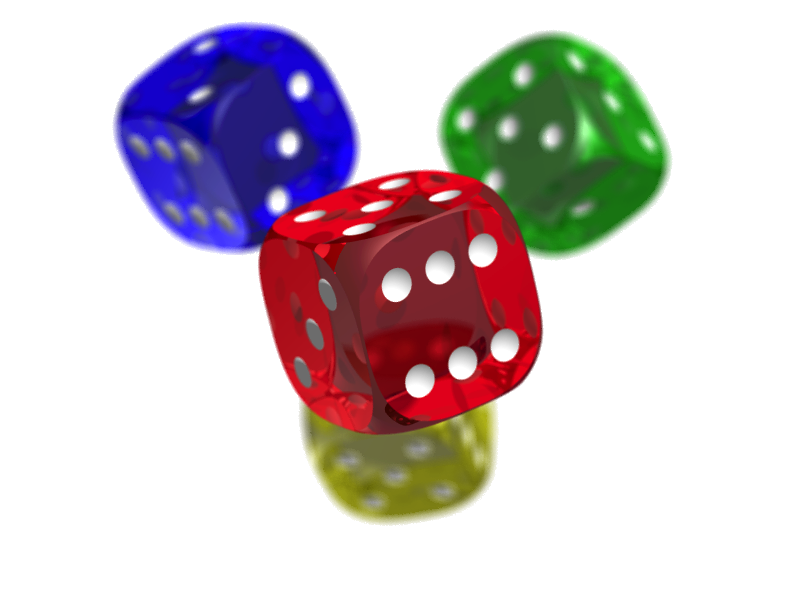
\includegraphics[width=0.30\textwidth]{images/dice.png}
        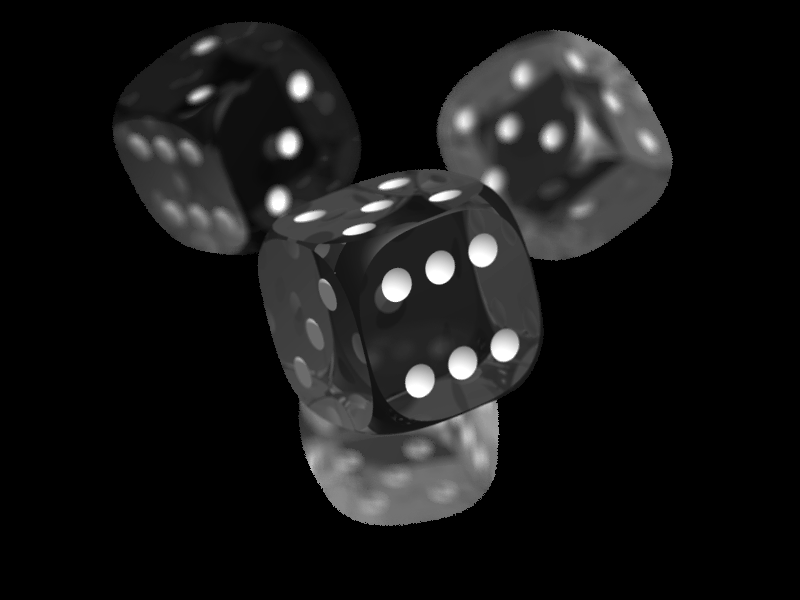
\includegraphics[width=0.30\textwidth]{images/results/grayscale-cv.dice.png}
        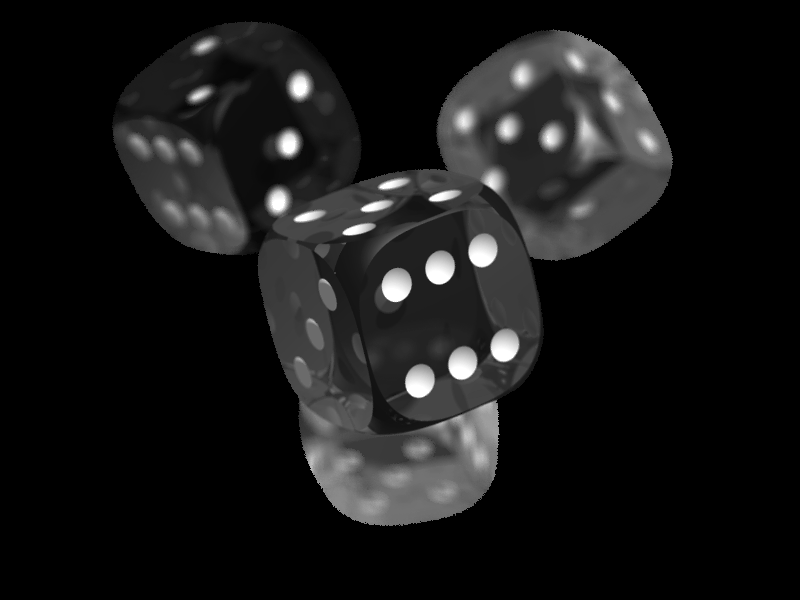
\includegraphics[width=0.30\textwidth]{images/results/grayscale-my.dice.png}

        
        \begin{center}
            \caption{Grayscale results of OpenCV (middle) and self-implemented  Algorithm (right)}            
        \end{center}

        \label{fig:grayscale1}
    \end{figure}
\end{frame}

\begin{frame}
    \frametitle{Grayscale - Performance 1}

    \begin{center}
    \begin{figure}[H]
        \centering

        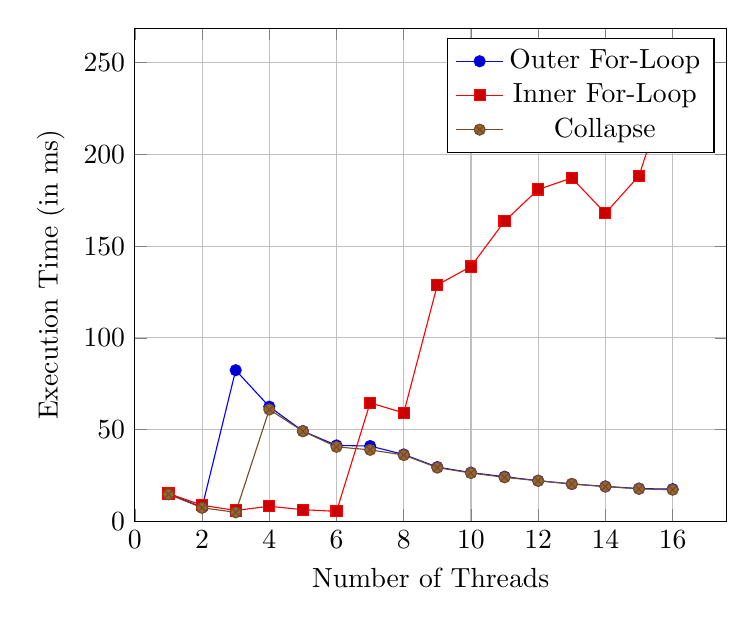
\begin{tikzpicture}
            \begin{axis}[
                title={},
                width=0.75\textwidth,
                xlabel={Number of Threads},
                ylabel={Execution Time (in ms)},
                xmin=0,
                ymin=0,
                grid=major
            ]
                \addplot coordinates {
                    (1,15.3049)(2,7.56055)(3,82.3768)(4,62.4837)(5,49.1818)(6,41.3728)(7,41.0167)(8,36.4371)(9,29.5454)(10,26.5446)(11,24.3035)(12,22.1388)(13,20.3482)(14,19.0172)(15,17.8612)(16,17.5258)
                };
                \addlegendentry{Outer For-Loop}

                \addplot coordinates {
                    (1,15.1618)(2,8.75195)(3,5.91315)(4,8.1956)(5,6.32605)(6,5.4254)(7,64.5677)(8,59.0846)(9,128.857)(10,138.879)(11,163.544)(12,180.893)(13,187.137)(14,167.894)(15,188.379)(16,244.342)
                };
                \addlegendentry{Inner For-Loop}       

                \addplot coordinates {
                    (1,14.7323)(2,7.3617)(3,4.90575)(4,60.9359)(5,49.1117)(6,40.5794)(7,38.9427)(8,36.1211)(9,29.2632)(10,26.3274)(11,23.971)(12,22.0927)(13,20.3762)(14,18.9155)(15,17.6862)(16,17.22)
                };
                \addlegendentry{Collapse}
            \end{axis}
        \end{tikzpicture}
        \caption{Grayscale Performance Tests dice.png}
    \end{figure}
\end{center}

\end{frame}

\begin{frame}
    \frametitle{Grayscale - Ergebnisse 2}

    \begin{itemize}
        \item dice\_large.png
        \item 1754 x 1554
        \item 1.5 MB
    \end{itemize}

    \hfill
    \hrule
    \hfill

    \begin{figure}[H]
        \centering
    
        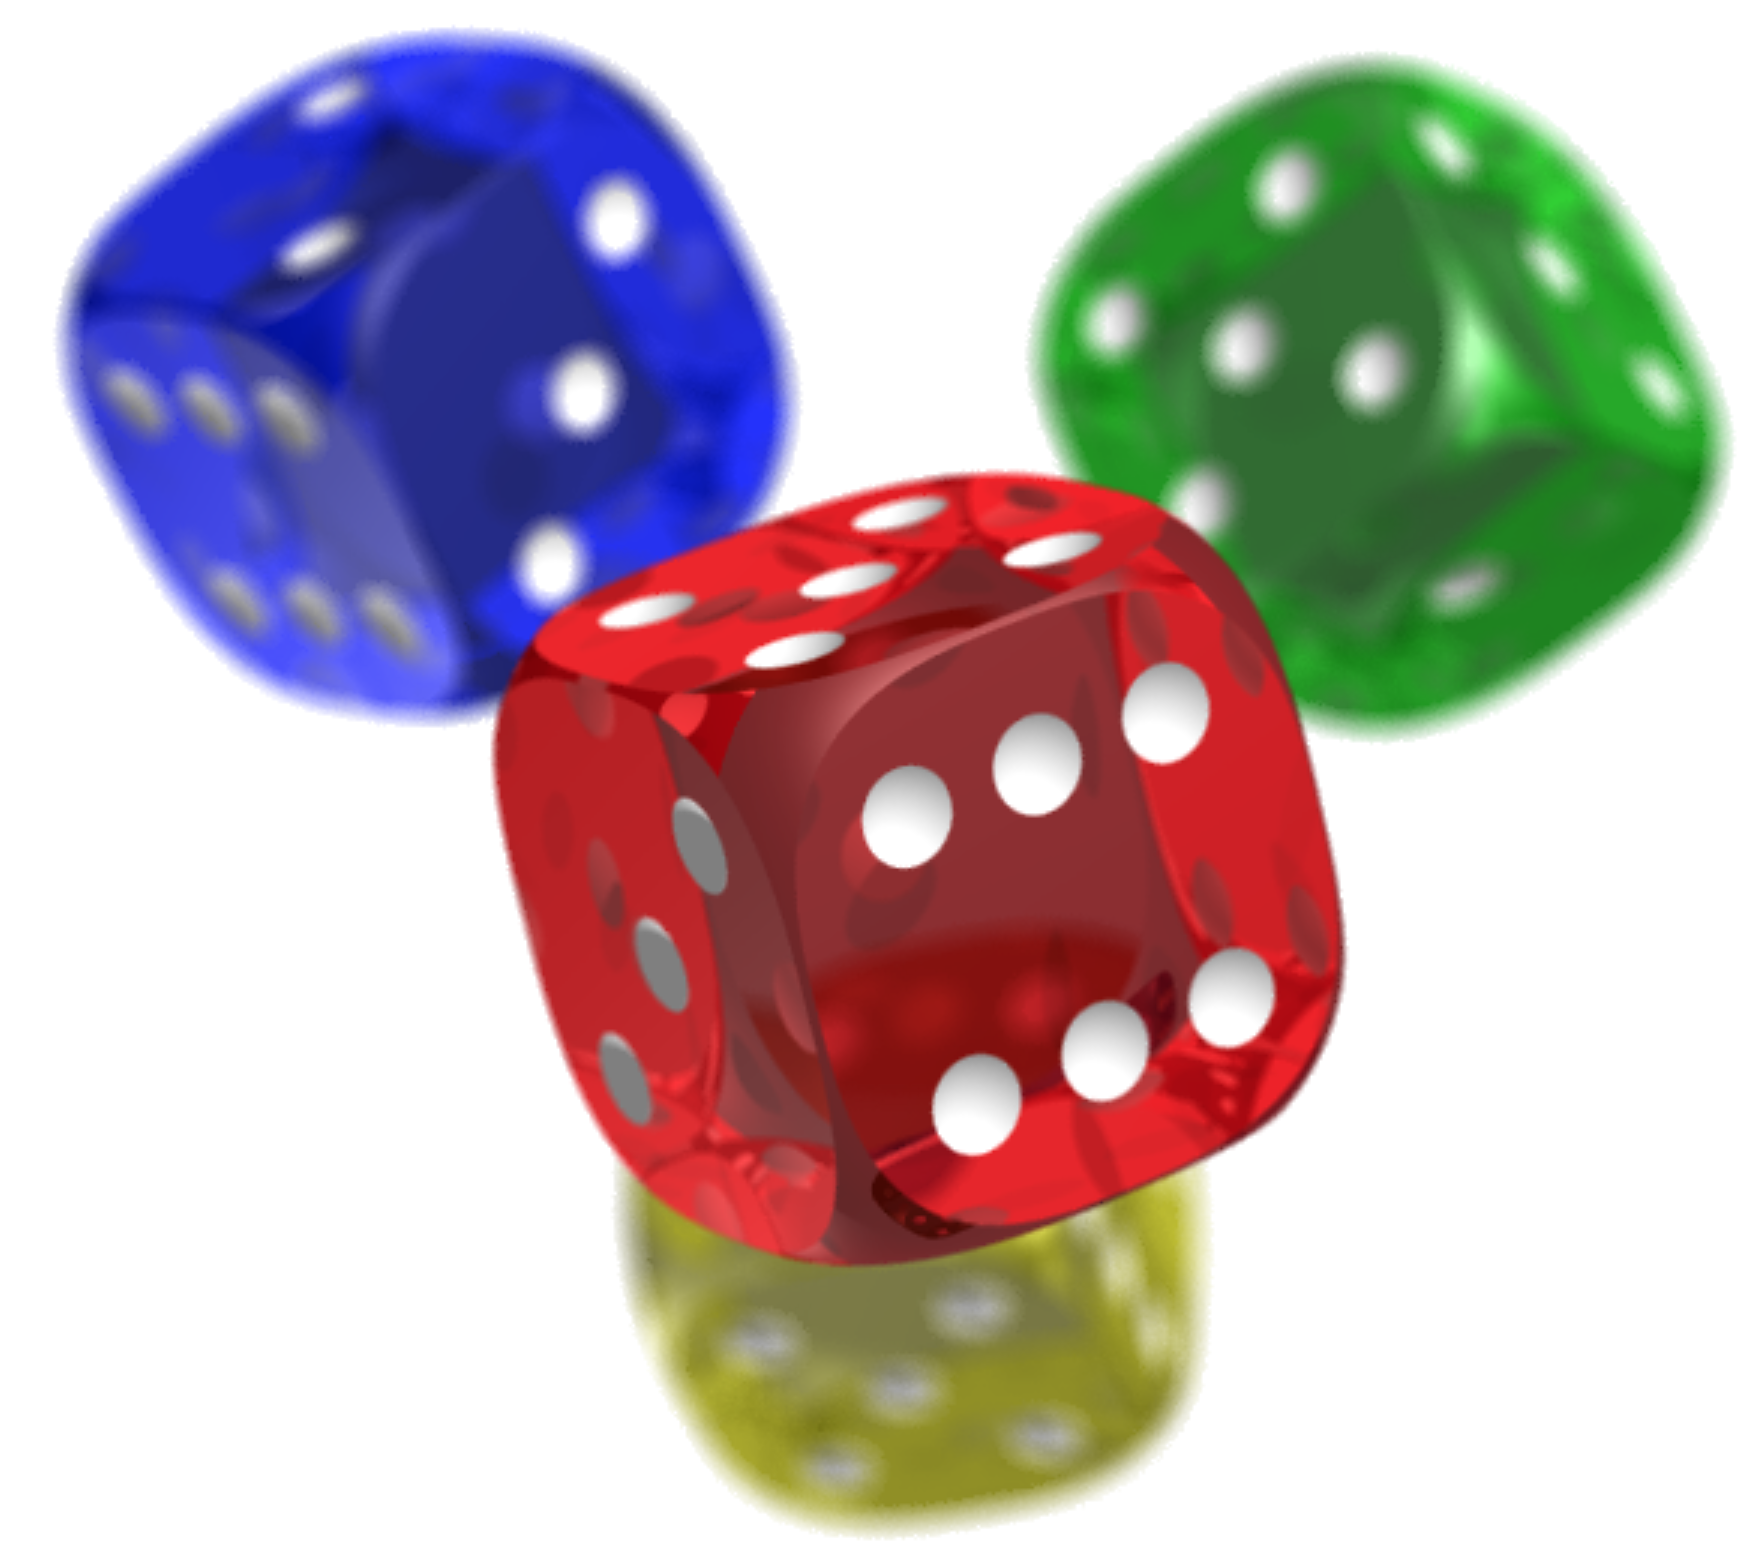
\includegraphics[width=0.30\textwidth]{images/dice_large.png}
        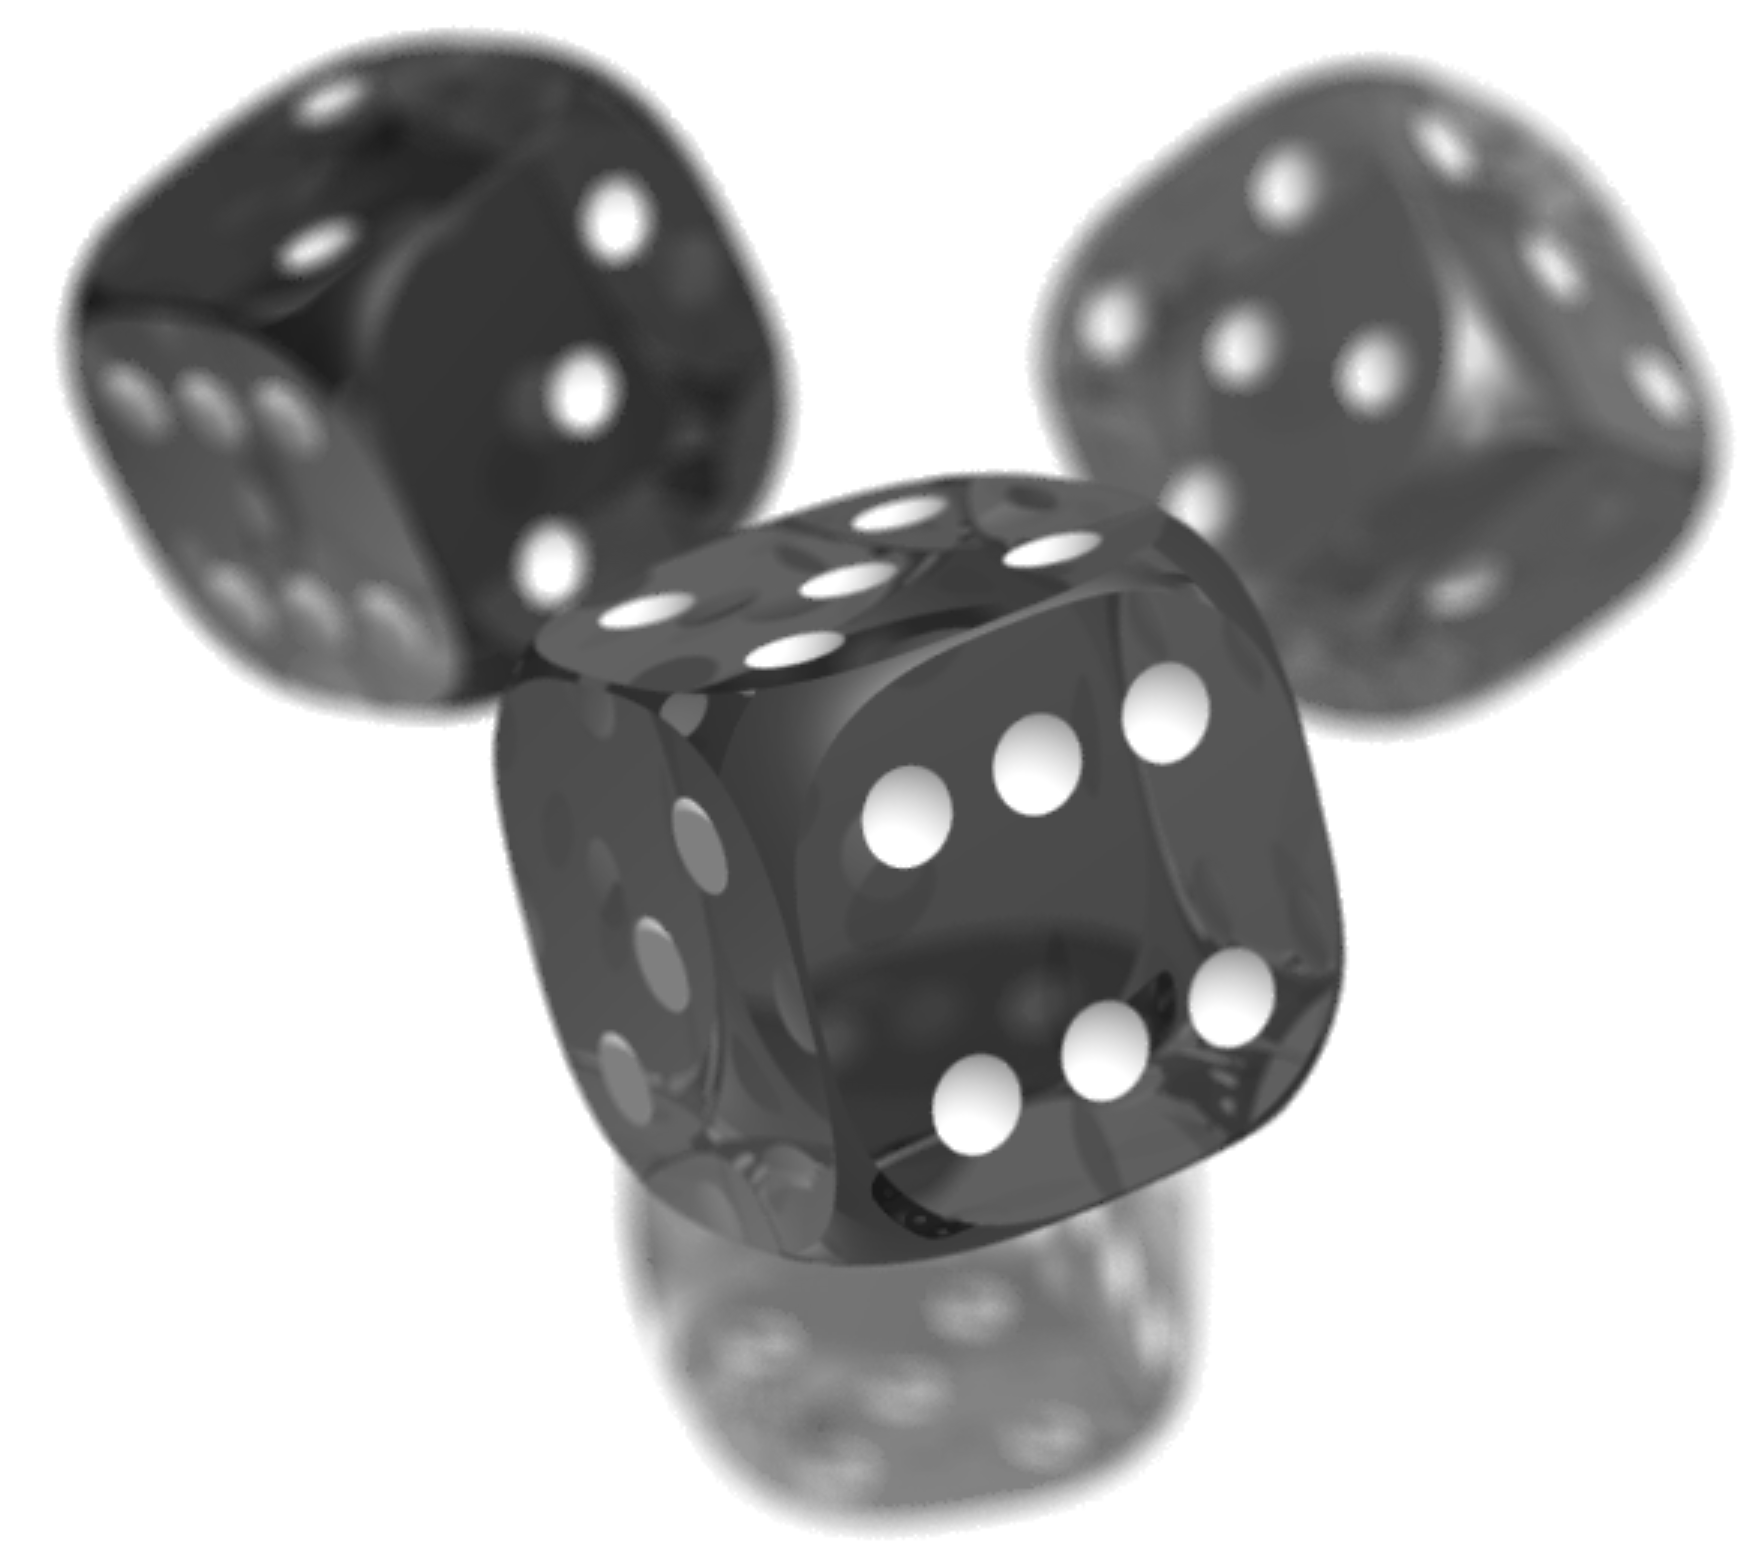
\includegraphics[width=0.30\textwidth]{images/results/grayscale-cv.dice_large.png}
        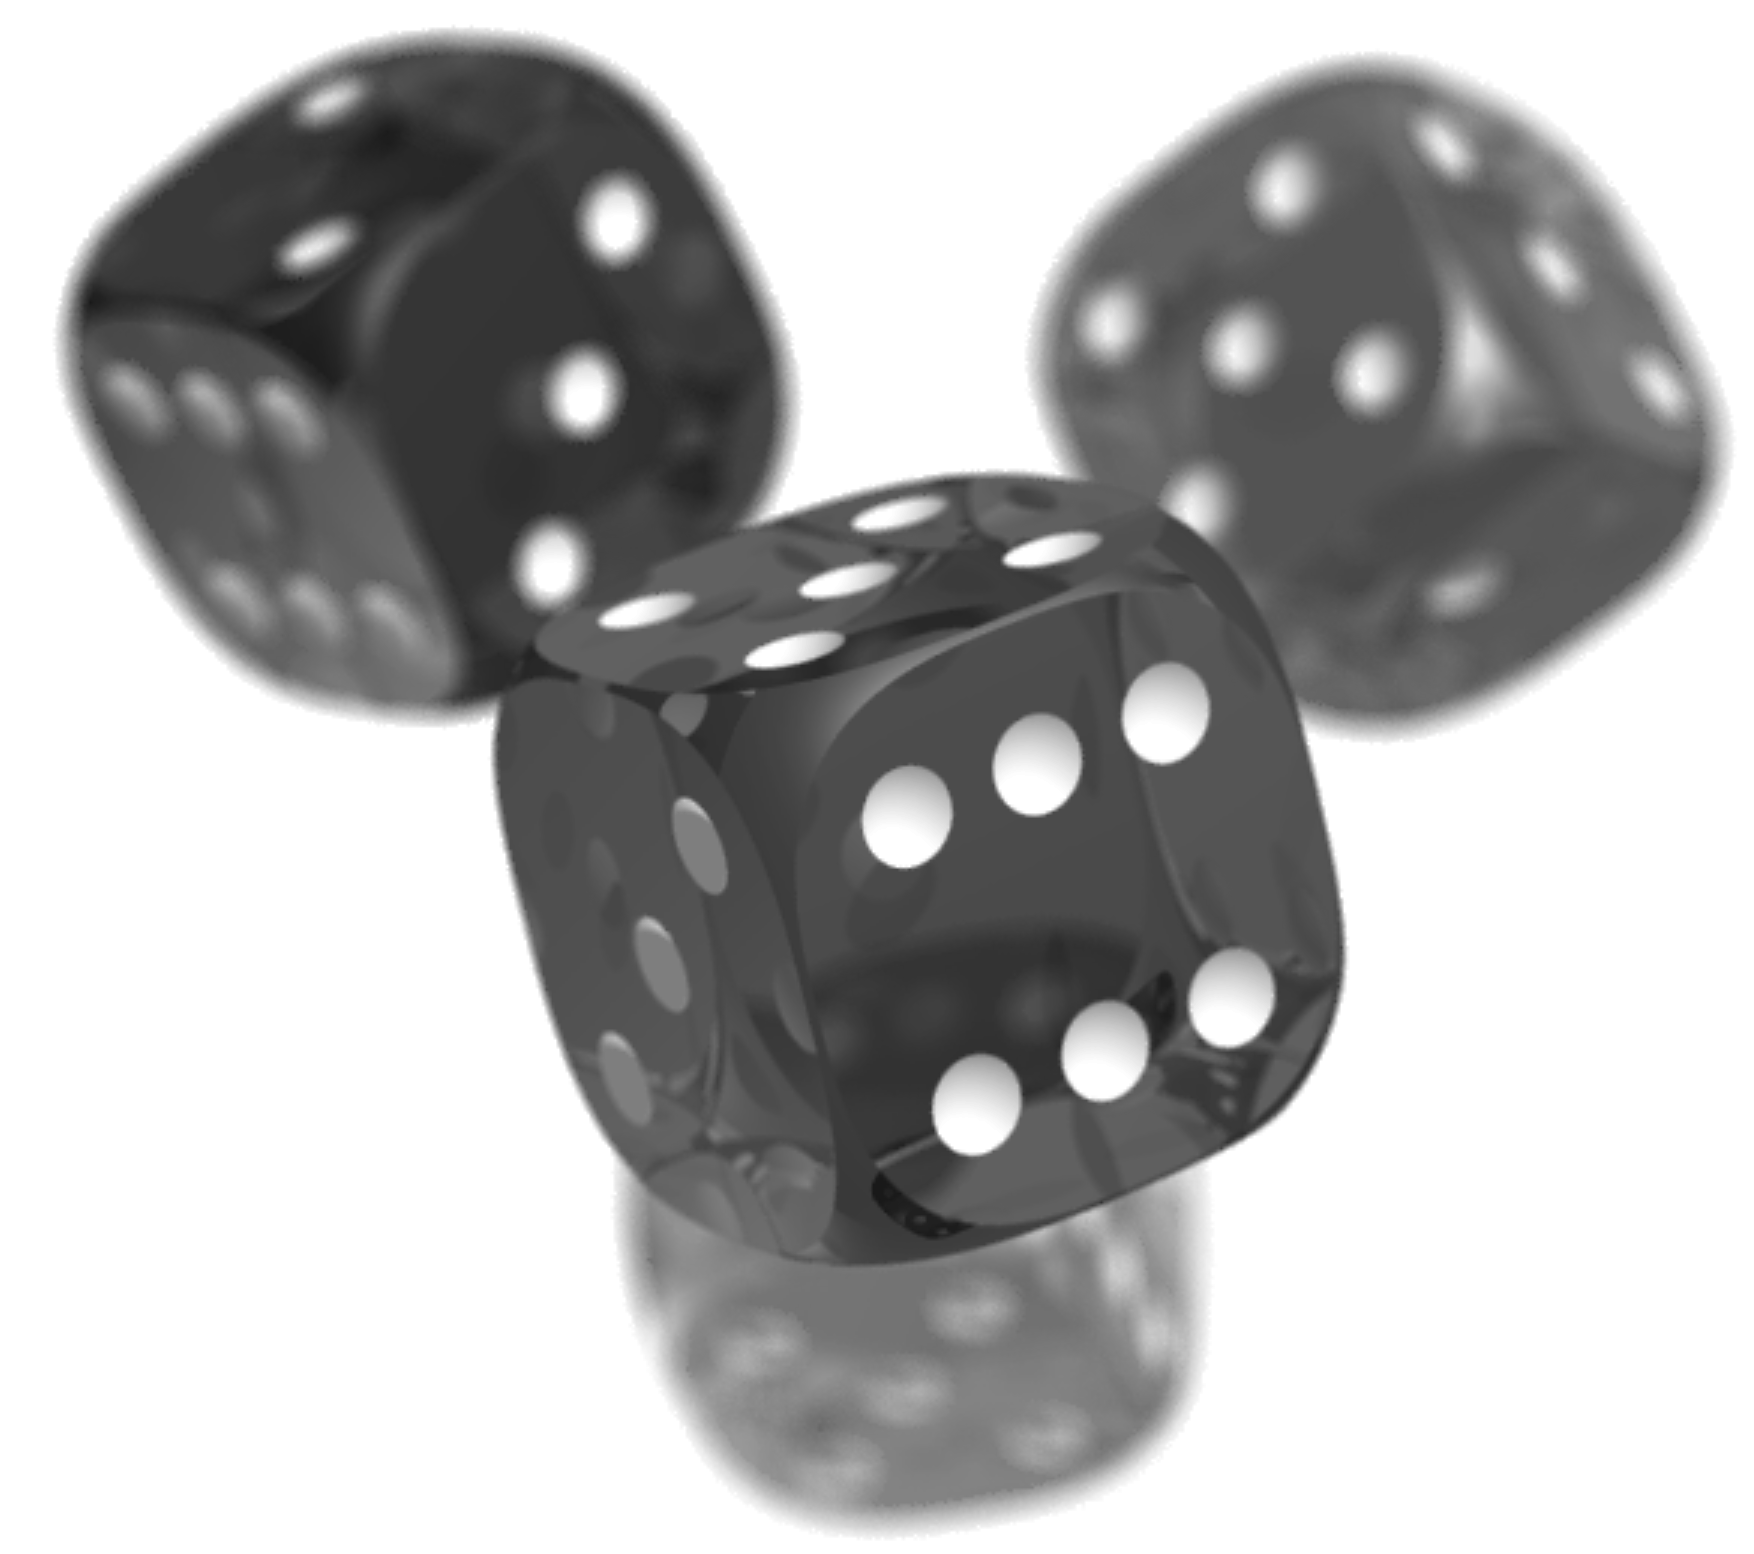
\includegraphics[width=0.30\textwidth]{images/results/grayscale-my.dice_large.png}

        
        \begin{center}
            \caption{Grayscale results of OpenCV (middle) and self-implemented  Algorithm (right)}            
        \end{center}

        \label{fig:grayscale2}
    \end{figure}
\end{frame}

\begin{frame}
    \frametitle{Grayscale - Performance 2}

    \begin{center}
    \begin{figure}[H]
        \centering

        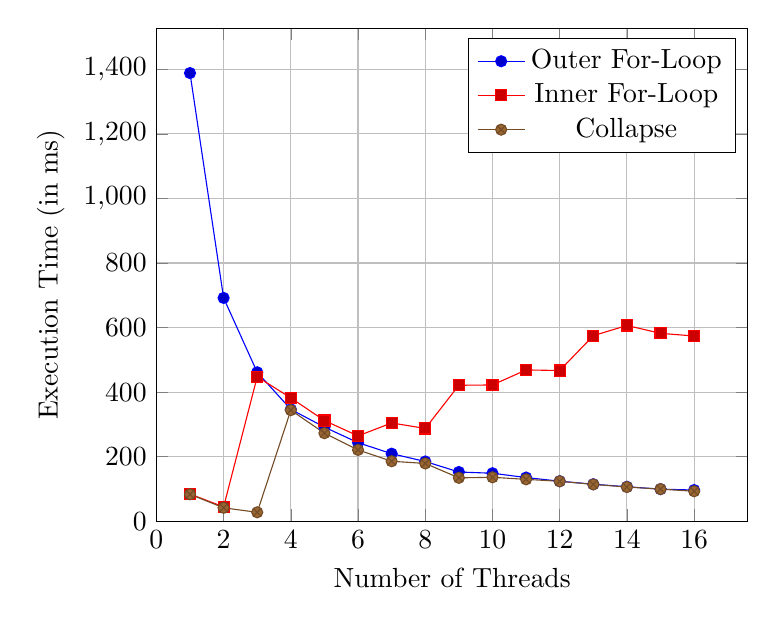
\begin{tikzpicture}
            \begin{axis}[
                title={},
                width=0.75\textwidth,
                xlabel={Number of Threads},
                ylabel={Execution Time (in ms)},
                xmin=0,
                ymin=0,
                grid=major
            ]
                \addplot coordinates {
                    (1,1388.14)(2,691.776)(3,461.453)(4,346.732)(5,291.6)(6,243.522)(7,209.415)(8,185.205)(9,152.677)(10,148.821)(11,135.525)(12,124.202)(13,114.814)(14,106.967)(15,99.6424)(16,96.8423)
                };
                \addlegendentry{Outer For-Loop}

                \addplot coordinates {
                    (1,84.6405)(2,44.5646)(3,447.501)(4,382.118)(5,311.966)(6,264.444)(7,304.552)(8,287.558)(9,421.305)(10,422.189)(11,468.759)(12,466.95)(13,574.857)(14,606.458)(15,582.076)(16,573.846)
                };
                \addlegendentry{Inner For-Loop}       

                \addplot coordinates {
                    (1,83.5909)(2,41.8099)(3,27.8556)(4,344.236)(5,272.88)(6,221.026)(7,185.961)(8,179.126)(9,134.584)(10,136.283)(11,129.925)(12,123.893)(13,114.326)(14,106.155)(15,99.6781)(16,93.0359)
                };
                \addlegendentry{Collapse}
            \end{axis}
        \end{tikzpicture}
        \caption{Grayscale Performance Tests dice\_large.png}
    \end{figure}
\end{center}

\end{frame}

\begin{frame}
    \frametitle{Grayscale - Ergebnisse 3}

    \begin{itemize}
        \item pnglogo-blk.png
        \item 1024 x 768
        \item 516 KB
    \end{itemize}

    \hfill
    \hrule
    \hfill

    \begin{figure}[H]
        \centering
    
        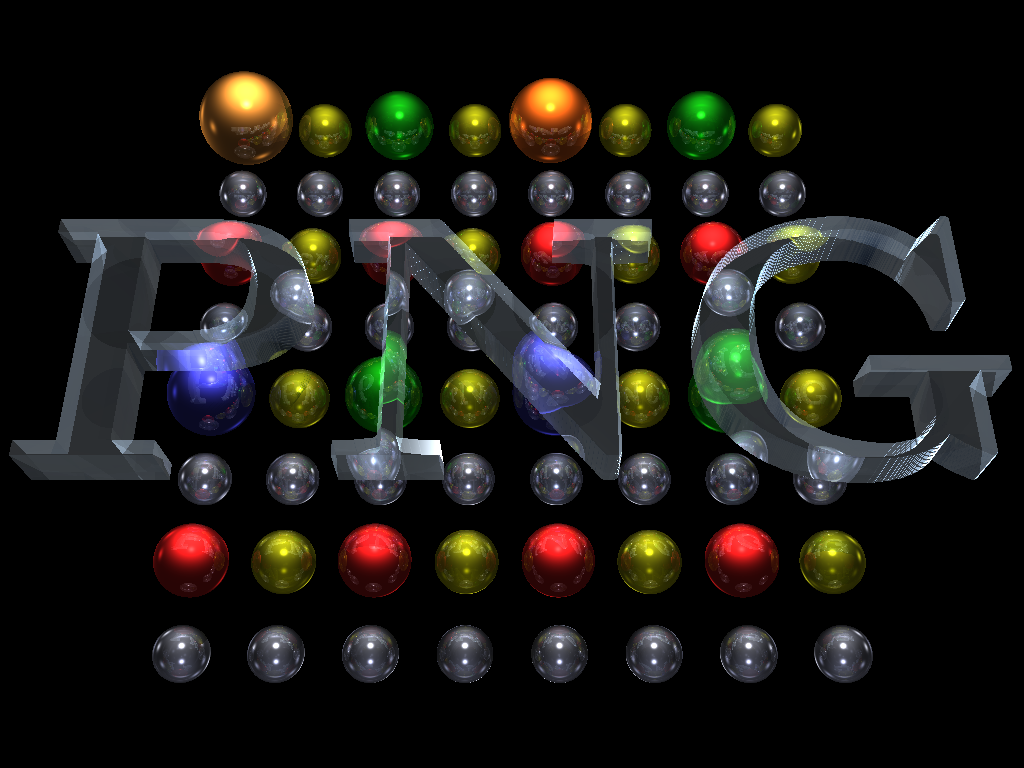
\includegraphics[width=0.30\textwidth]{images/pnglogo-blk.png}
        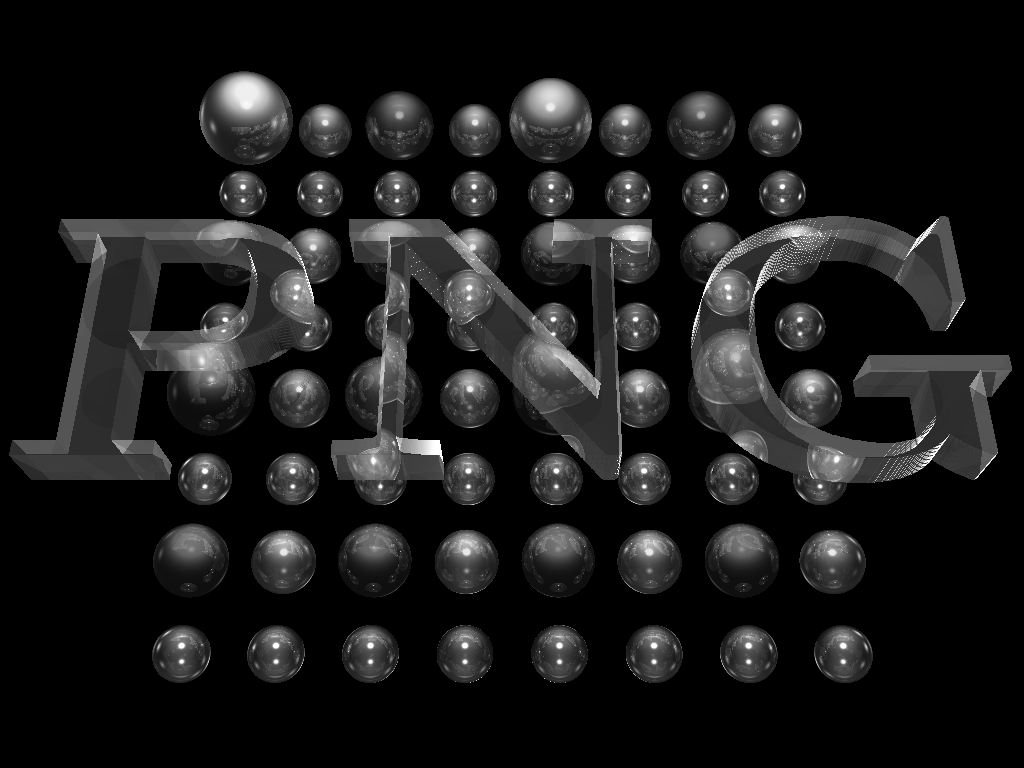
\includegraphics[width=0.30\textwidth]{images/results/grayscale-cv.pnglogo-blk.png}
        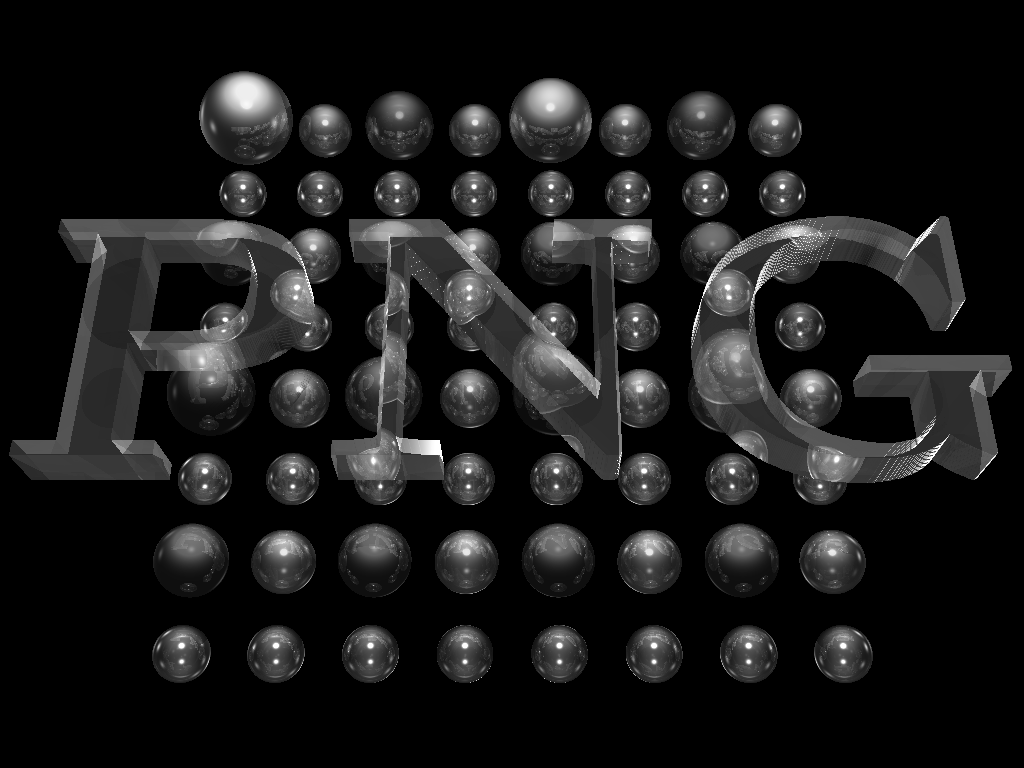
\includegraphics[width=0.30\textwidth]{images/results/grayscale-my.pnglogo-blk.png}

        
        \begin{center}
            \caption{Grayscale results of OpenCV (middle) and self-implemented  Algorithm (right)}            
        \end{center}

        \label{fig:grayscale3}
    \end{figure}
\end{frame}

\begin{frame}
    \frametitle{Grayscale - Performance 3}

    \begin{center}
    \begin{figure}[H]
        \centering

        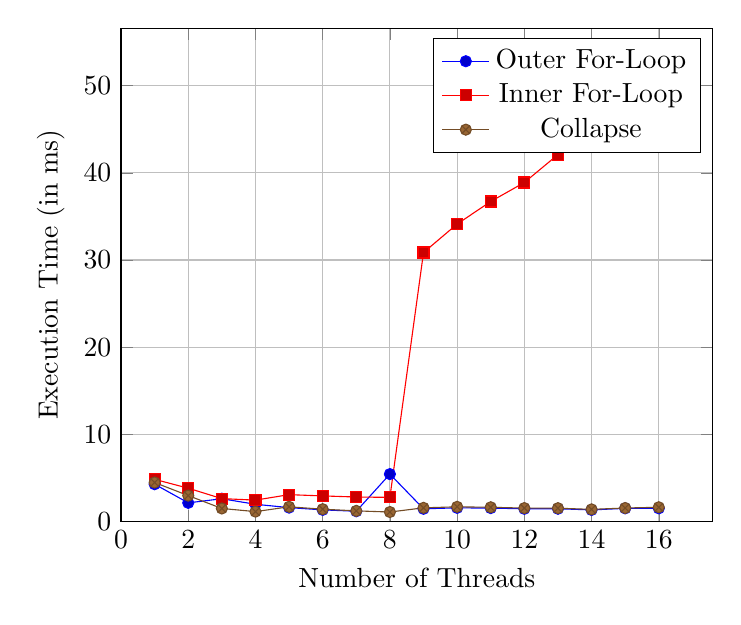
\begin{tikzpicture}
            \begin{axis}[
                title={},
                width=0.75\textwidth,
                xlabel={Number of Threads},
                ylabel={Execution Time (in ms)},
                xmin=0,
                ymin=0,
                grid=major
            ]
                \addplot coordinates {
                    (1,4.25925)(2,2.11895)(3,2.5918)(4,1.9537)(5,1.572)(6,1.31315)(7,1.15475)(8,5.41915)(9,1.43565)(10,1.5453)(11,1.5184)(12,1.4348)(13,1.44295)(14,1.30675)(15,1.48805)(16,1.48985)
                };
                \addlegendentry{Outer For-Loop}

                \addplot coordinates {
                    (1,4.8171)(2,3.7998)(3,2.60445)(4,2.43305)(5,3.0599)(6,2.9158)(7,2.7888)(8,2.74855)(9,30.8562)(10,34.1217)(11,36.713)(12,38.8938)(13,42.0953)(14,49.7418)(15,48.6)(16,51.4584)
                };
                \addlegendentry{Inner For-Loop}       

                \addplot coordinates {
                    (1,4.4527)(2,2.95205)(3,1.47325)(4,1.11305)(5,1.66655)(6,1.3907)(7,1.1971)(8,1.06665)(9,1.5488)(10,1.66275)(11,1.61175)(12,1.5165)(13,1.5057)(14,1.3701)(15,1.5257)(16,1.6131)
                };
                \addlegendentry{Collapse}
            \end{axis}
        \end{tikzpicture}
        \caption{Grayscale Performance Tests pnglogo-blk.png}
    \end{figure}
\end{center}

\end{frame}